\documentclass{report}
\usepackage[utf8]{inputenc}
\usepackage{amsmath}
\usepackage{amsthm}
\usepackage{mathtools,xparse}
\usepackage{amsfonts}
\usepackage[usenames,dvipsnames]{color}
\usepackage{tikz}
\usepackage{biblatex} %Imports biblatex package
\addbibresource{references.bib} %Import the bibliography file
\newtheorem{theorem}{Theorem}[section]
\newtheorem{corollary}{Corollary}[theorem]
\newtheorem{lemma}[theorem]{Lemma}
\usepackage[colorlinks=true]{hyperref}
\title{Stat RL}
\author{Chufan Chen}
\date{September 2022}

\begin{document}
\maketitle
\tableofcontents
\chapter{Preliminaries}

\section{Markov Decision Process}
In reinforcement learning, the interactions between the agent and the environment are often described
by a Markov Decision Process (MDP)\cite{Puterman2005MarkovProgramming}, specified by: 
\begin{itemize}
    \item State space S.
    \item Action space A.
    \item Transition function/kernel P: $S \times A \rightarrow \Delta(S)$, where $\Delta(S)$ is the space of probability distributions over S (i.e., the probability simplex). $P(s'\mid s, a)$ is the probability of transitioning into state s' upon taking action a in state s.
    \item Reward function R: $ S \times A \rightarrow [0,R_{max}]$, where $R_{max} > 0$ is a constant. $R(s, a)$ is the immediate reward associated with taking action a in state s.
    \item Discount factor $\gamma \in [0,1)$, which defines a horizon for the problem
\end{itemize}

\subsection{Shift of rewards}
Why it is sufficient to define reward as nonnegative?\\
Consider two MDPs $M=(S,A,P,R,\gamma)$ and $M=(S,A,P,R',\gamma)$, which only differ in their reward functions. Moreover, we have for any $s \in S,a\in A$, \[R(s,a)=R'(s,a)+c\], where c is a universal constant that does not depend on s or a. Then these two MDPs in some particular sense are equivalent to each other. For any policy $\pi$, let $V_M^{\pi}$ denotes its value function in M and $V_{M'}^{\pi}$, denote its value function in M'. For any $s\in S$, \[V_M^{\pi}=V_{M'}^{\pi}+\frac{c}{1-\gamma}\]. The reward shift doesn't change the order of the optimality of the policy and $\forall \pi_1, \pi_2, V_{M}^{\pi_1}-V_{M}^{\pi_2}=V_{M'}^{\pi_1}-V_{M'}^{\pi_2}$. In a bounded reward, the constant shift doesn't matter. We can make the assumption that rewards lie in $[0, R_{max}]$ without loss of generality.

\subsection{Interaction protocol}
In a given MDP $M=(S,A,P,R,\gamma)$, the agent interacts with the environment according to the following protocol: the agent starts at some state $s_1$; at each time step $t = 1, 2, \hdots $, the agent takes an action $a_t \in A$, obtain the immediate reward $r_t=R(s_t,a_t)$, and observes the next state $s_{t+1}$ sampled from $P(s_t, a_t)$ , or $s_{t+1}\sim P(s_t,a_t)$. The interaction record \[ \tau=(s_1,a_1,r_1,s_2,\hdots,s_{H+1})\] is called a trajectory of length H. \\
In some situations, it is necessary to specify how the initial state $s_1$ is generated. We consider $s_1$ sampled from an initial distribution $d_0 \in \Delta(S)$. When $d_0$ is of importance to the discussion, we include it as part of the MDP definition, and write $M = (S, A, P, R, \gamma, d_0)$.

\subsection{Finite-horizon MDPs}
Without explicit mention, we assume MDP as infinite-horizon discounted for its mathematical convenience. But finite-horizon MDP is more natural in some sense. We cut down the trajectory after H steps, where H is a predefined constant That is, with the same generative process of trajectories, we now consider return to be defined as \[E[\sum_{h=1}^{H} r_h]\]. A finite-horizon MDP is usually specified as $M=(S,A,P,R,H,d_0)$, where H is the episode length (or horizon) and $d_0 \in \Delta(S)$ is the initial state distribution (from which $s_1$ is drawn).  Note that there is no discount factor in finite-horizon MDP. Discount factor is only introduced only for mathematical convenience. It gives you two properties:
\begin{enumerate}
    \item Stationarity. The optimal policy and value function don't depend on the time-step. It only depends on which state you're in.
    \item You can add up an infinite number of rewards that always converge.
\end{enumerate}
Optimal policies in finite-horizon MDPs are generally non-stationary, i.e., you need to look at both the current state and the number of steps remaining to make an optimal decision. In finite-horizon MDPs, you only add up a finite number(H) of rewards, so it doesn't blow up anyway. If we add a constant shift c, $E[\sum_{h=1}^{H} (r_h+c)]=E[\sum_{h=1}^{H} r_h] + cH$. For the value function for every state, consider the following formulation: State space S is layered by a disjoint H subset, a state in each subset can only appear in a particular time-step: $S=\cup_{h=1}^{H}S_h$. $\forall s \in S_h$, $V_{M'}^{\pi}(s,h)=V_{M}^{\pi}+c(H-h+1)$.


\tikzset{every picture/.style={line width=0.75pt}} %set default line width to 0.75pt        

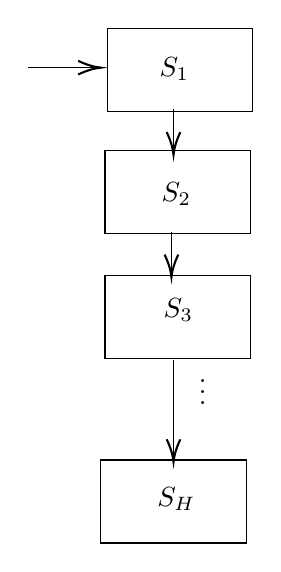
\begin{tikzpicture}[x=0.75pt,y=0.75pt,yscale=-1,xscale=1]
%uncomment if require: \path (0,300); %set diagram left start at 0, and has height of 300

%Shape: Rectangle [id:dp026637602652964] 
\draw   (222,12) -- (292,12) -- (292,52) -- (222,52) -- cycle ;
%Shape: Rectangle [id:dp5134797540715976] 
\draw   (221,71) -- (291,71) -- (291,111) -- (221,111) -- cycle ;
%Shape: Rectangle [id:dp49488356415499957] 
\draw   (221,131) -- (291,131) -- (291,171) -- (221,171) -- cycle ;
%Shape: Rectangle [id:dp6001486456175422] 
\draw   (219,220) -- (289,220) -- (289,260) -- (219,260) -- cycle ;
%Straight Lines [id:da3116448871709194] 
\draw    (254,51) -- (254,71) ;
\draw [shift={(254,73)}, rotate = 270] [color={rgb, 255:red, 0; green, 0; blue, 0 }  ][line width=0.75]    (10.93,-3.29) .. controls (6.95,-1.4) and (3.31,-0.3) .. (0,0) .. controls (3.31,0.3) and (6.95,1.4) .. (10.93,3.29)   ;
%Straight Lines [id:da0970380224865115] 
\draw    (253,110) -- (253,130) ;
\draw [shift={(253,132)}, rotate = 270] [color={rgb, 255:red, 0; green, 0; blue, 0 }  ][line width=0.75]    (10.93,-3.29) .. controls (6.95,-1.4) and (3.31,-0.3) .. (0,0) .. controls (3.31,0.3) and (6.95,1.4) .. (10.93,3.29)   ;
%Straight Lines [id:da09351815358456728] 
\draw    (254,172) -- (254,219) ;
\draw [shift={(254,221)}, rotate = 270] [color={rgb, 255:red, 0; green, 0; blue, 0 }  ][line width=0.75]    (10.93,-3.29) .. controls (6.95,-1.4) and (3.31,-0.3) .. (0,0) .. controls (3.31,0.3) and (6.95,1.4) .. (10.93,3.29)   ;
%Straight Lines [id:da3881071800899032] 
\draw    (184,31) -- (217,31) ;
\draw [shift={(219,31)}, rotate = 180] [color={rgb, 255:red, 0; green, 0; blue, 0 }  ][line width=0.75]    (10.93,-3.29) .. controls (6.95,-1.4) and (3.31,-0.3) .. (0,0) .. controls (3.31,0.3) and (6.95,1.4) .. (10.93,3.29)   ;

% Text Node
\draw (246,25) node [anchor=north west][inner sep=0.75pt]   [align=left] {$\displaystyle S_{1}$};
% Text Node
\draw (247,85) node [anchor=north west][inner sep=0.75pt]   [align=left] {$\displaystyle S_{2}$};
% Text Node
\draw (248,141) node [anchor=north west][inner sep=0.75pt]   [align=left] {$\displaystyle S_{3}$};
% Text Node
\draw (245,232) node [anchor=north west][inner sep=0.75pt]   [align=left] {$\displaystyle S_{H}$};
% Text Node
\draw (265,172) node [anchor=north west][inner sep=0.75pt]   [align=left] {$\displaystyle \vdots$};


\end{tikzpicture}

\subsection{Indefinite-horizon MDPs}
Here is yet another formulation, which is similar to finite-horizon MDPs except that the episode length H can vary: A subset of the state space $S_{term} \subset S$ are considered terminal, and an episode $s_1,a_1,r_1,s_2,a_2,r_2,\hdots$ keeps rolling out until we first visit a terminal state, $s_H \in S_{term}$. In general, the length of the episode, H, is a random variable or a function of policy.The value is still defined as $E[\sum_{h=1}^{H}r_h]$. Examples include the stochastic shortest paths. As an another example, consider  consider a navigation task where the goal is to get to the destination state as soon as possible. Let’s model it as an indefinite-horizon MDP: reward is -1 per step, and the process terminates whenever we reach the destination. It is clear then the return of a policy is the negative expected total number of steps towards destination. If we add +2 to all rewards, we're not trying to terminate the MDP as soon as possible.
You cannot shift reward arbitrary because the length of trajectory depends on how you behave. \\
Suppose there exists some constant $H_0$ such that $H \leq H_0$ holds almost surely for an indefinite-horizon MDP. By adding an absorbing state which gives 0 reward and loops in itself. After padding the MDP with the dummy state, you can shift reward both in original MDP states and dummy states.

\subsection{Non-stationary dynamics}
So far all our definitions consider stationary dynamics, that is, the transition function only depends on the state and action, and does not depend on the time step. A finite-horizon MDP with non-stationary dynamics (and reward function) is a generalization: $M=(S,A,\{P_H\}_{h=1}^H,H,d_0)$, where $s_1\sim d_0,s_{h+1}\sim P_h(s_h,a_h)$ and $r_{h+1}=R_h(s_h,a_h)$. That is, the transition rule and reward function can change as time elapses. Stationary MDP is a special case of non-stationary MDP, $S_1=S_2=\hdots=S_H, P_1=P_2=\hdots=P_H$. On the other hand, non-stationary MDP is also a special case of stationary MDP, we can augment state space $s'=(s,h)$. Now the state space is H time larger, the benefit is that we can have a single function $P((s',h+1)\mid (s',h),a)$ and not every function for every time-step. By definition, $P((s',h')\mid (s,h),a)=0$ if $h'-h \neq 1$.
\subsection{Policy and value}
A (deterministic and stationary) policy $\pi:S\rightarrow A$ specifies a decision-making strategy in which the agent chooses actions adaptively based on the current state, i.e., $a_t = \pi(s_t)$. More generally, the agent may also choose actions according to a stochastic policy $\pi:S\rightarrow \Delta(A)$, and with a slight abuse of notation we write $a_t \sim \pi(s_t)$. A deterministic policy is its special case when $\pi(s)$ is a point mass for all $s\in S$. \\
The goal of the agent is to choose a policy $\pi$ to maximize the expected discounted sum of rewards, or value:
\begin{equation}
    E[\sum_{t=1}^{\infty}\gamma^{t-1}r_t\mid \pi,s_1].
\end{equation}
The expectation is with respect to the randomness of the trajectory, that is, the randomness in state transitions and the stochasticity of $\pi$. Notice that, since $r_t$ is nonnegative and upper bounded by $R_{max}$, we have
\begin{equation}
    0 \leq \sum_{t=1}^{\infty}\gamma^{t-1}r_t \leq \sum_{t=1}^{\infty}\gamma^{t-1}R_{max}=\frac{R_{max}}{1-\gamma}.
\end{equation}
Hence, the discounted sum of rewards (or the discounted return) along any actual trajectory is always
bounded in the range $[0,\frac{R_{max}}{1-\gamma}]$, and so is its expectation of any form. This fact will be important when we later analyze the error propagation of planning and learning algorithms.\\
Note that for a fixed policy, its value may differ for a different choice of $s_1$, and we define the value function $V_{M}^{\pi}:S \rightarrow \mathbb{R}$ as 
\[
V_{M}^{\pi}(s)=E[\sum_{t=1}^{\infty}\gamma^{t-1}r_t\mid \pi, s_1=s],
\]
which is the value obtained by following policy $\pi$ starting at state s. Similarly, we define the action-value(or Q-value) function $Q_M^{\pi}:S\times A \rightarrow \mathbb{R}$ as 
\[
Q_M^{\pi}(s,a)=E[\sum_{t=1}^{\infty}\gamma^{t-1}r_t\mid \pi, s_1=s,a_1=a].
\]
Henceforth, the dependence of any notation on M will be made implicit whenever it is clear from the context.

\subsection{Bellman equation for policy evaluation}
Based on the principles of dynamic programming, $V^{\pi}$ and $Q^{\pi}$ can be computed using the following bellman equation for policy evaluation: $\forall s\in S, a \in A$
\begin{equation} \label{eq1}
\begin{split}
V^{\pi}(s) & = E[\sum_{t=1}^{\infty}\gamma^{t-1}r_t \mid s_1=s,\pi] \\
          & = Q(s, \pi(s)) \\ 
          & = R(s,\pi(s))+\gamma E_{s' \sim P(s,a)}[V^{\pi}(s')] \\
          & = R(s,\pi(s))+\gamma \sum_{s'\in S}P(s' \mid s,\pi(s))V^{\pi}(s') 
\end{split}
\end{equation}
\begin{equation} \label{eq2}
\begin{split}
    Q^{\pi}(s,a) & = R(s,a)+\gamma E_{s'\sim P(s,a)}[V^{\pi}(s')] \\
                & =  R(s,a)+\gamma E_{s'\sim P(s,a)}[Q^{\pi}(s', \pi(s'))]           
\end{split}
\end{equation}
In $Q(s, \pi(s))$ and $R(s,\pi(s))$ we treat $\pi$ as a deterministic policy for brevity, and for stochastic policies this shorthand should be interpreted as $E_{a\sim\pi(s)}[Q^{\pi}(s,a)]$ and $E_{a\sim\pi(s)}[R^{\pi}(s,a)]$.\\
If we assume S and A are finite, upon fixing an arbitrary order of states and actions, we can rewrite \ref{eq1} and \ref{eq2} in matrix form and derive an analytical solution for $V^{\pi}$ and $Q^{\pi}$ using linear algebra as below. Define:
\begin{itemize}
    \item $V^{\pi}$ as the $\mid S\mid \times 1$ vector $[V^{\pi}(s)]_{s\in S}$
    \item $R^{\pi}$ as the reward vector for policy $\pi$ with dimension $\mid S \mid \times 1$, whose s-th entry is \[[R^{\pi}]_s=E_{a\sim\pi(s)}[R(s,a)]\]. For deterministic policy $\pi$, \[
        [R^{\pi}]_s=R(s,\pi(s))
    \].
    \item $P^{\pi}$ as the matrix $[P(s'\mid s,\pi(s))]_{s\in S,s'\in S}$, whose ($s,s'$)-th entry is \[[P^{\pi}]_{s,s'}=E_{a\sim\pi(s)}[P(s'\mid s,a)]\]. Similarly, for deterministic policy $\pi$, \[
        [P^{\pi}]_{s,s'}=P(s'\mid s,\pi(s))
    \].In fact, this matrix describes a Markov chain induced by MDP M and policy $\pi$. Its s-th row is the distribution over next-states upon taking actions according to $\pi$ at state s , which we also write as $[P(s,\pi)]^{\top}$.
\end{itemize}
Then from \ref{eq1} we have
\begin{equation}
    \forall s, [V^{\pi}]_s=[R^{\pi}]_s+\gamma \langle P(s,\pi),V^{\pi}\rangle
\end{equation}
\[
V^{\pi} =  R^{\pi}+\gamma P^{\pi}V^{\pi}
\]
When it comes to Q function, the notations are slightly different. Define:
\begin{itemize}
    \item $Q^{\pi}$ as the $\mid S \times A \mid \times 1$ vector $[Q^{\pi}(s,a)]_{s\in S,a\in 
 A}$
    \item $R$ as the reward vector with dimension $\mid S \times A \mid \times 1$, whose (s,a)-th entry is \[[R]_{s,a}=R(s,a)\]. 
    \item $P$ as the $|S \times A|\times |S|$ matrix $[P(s'\mid s,a)]_{s\in S,s'\in S}$, whose ($(s,a),s'$)-th entry is \[[P]_{(s,a),s'}=P(s'\mid s,a)\]. 
\end{itemize}
From \ref{eq2} we have:
\begin{equation}
    \forall s,a, [Q^{\pi}]_{(s,a)}=[R]_{(s,a)}+\gamma \langle [P]_{(s,a)}, V^{\pi}\rangle
\end{equation}
\[
Q^{\pi}=R+\gamma PV^{\pi}
\]
\begin{align*}
V^{\pi} &=  R^{\pi}+\gamma P^{\pi}V^{\pi} \\ 
(I-\gamma P^{\pi})V^{\pi} &=  R^{\pi} \\
V^{\pi} &= (I-\gamma P^{\pi})^{-1}R^{\pi} \\
Q^{\pi}&=R+\gamma P(1-\gamma P^{\pi})^{-1}R^{\pi}
\end{align*}   
Now we notice that matrix$(I_{\mid S \mid}-\gamma P^{\pi})$ is always invertible.  
Ways to prove a matrix $A$ is invertible:
\begin{enumerate}
    \item The null space/kernel of  A  is trivial. That is $Ax=0 \iff x=0$.
    \item $0$ is not an eigenvalue.
    \item The determinant of $A$ is nonzero.
    \item If at any point of the Gauss-Jordan process on $A$ you can get it into a reduced row echelon form. Likewise,  $A$ is not invertible if you get a row or column of all zeros at some point while using Gauss-Jordan.
\end{enumerate}
Here we use the first method:
\begin{equation}
\begin{split}
    \Vert(I-\gamma P^{\pi})x\Vert_{\infty}
    &\geq \Vert Ix \Vert_{\infty} -\gamma \Vert P^{\pi} x \Vert_{\infty} \text{(triangular inequality for norms)} \\
    &\geq \Vert Ix \Vert_{\infty} - \gamma \Vert x \Vert_{\infty} \text{(each element of $P^{\pi}x$ is a convex average of x)} \\
   & = (1-\gamma)\Vert x \Vert_{\infty} \geq 0
\end{split}
\end{equation}
So we can conclude that 
\begin{equation}
    V^{\pi}=(I-\gamma P^{\pi})^{-1}R^{\pi}.
\end{equation}
Why does the infinity norm work here?\\
$P$ is a row-stochastic matrix. 
Hölder's inequality tells us that L1-norm and infinity norm are dual pairs.

\subsection{State occupancy}
\[(I-\gamma P^{\pi})^{-1}\] is a matrix, where each row (indexed by s) is the discounted state occupancy $d_s^{\pi}$, whose s'-th entry is \[d_s^{\pi}(s')=E[\sum_{t=1}^{\infty}\gamma^{t-1} \mathbb{1}[s_t=s'] \mid s_1=s,\pi]\]. It is similar to the notion of occupancy distribution/stationary distribution in the ergodic Markov chain.
\begin{enumerate}
    \item Each row is like a distribution vector except that the entries sum up to $\frac{1}{1-\gamma}$. Let $\eta_{s}^{\pi}=(1-\gamma)d_s^{\pi}$ denote the normalized vector.
    \item $V^{\pi}(s)$ is the dot product between $d_s^{\pi}$ and reward vector.
    \item Can also be interpreted as the value function of the indicator reward function.
\end{enumerate}

\subsection{Optimality}
For infinite-horizon discounted MDPs, there always exists a 
stationary and deterministic policy that is optimal for all starting states simultaneously. Let $\pi^*$ denote this optimal policy, and $V^* := V^{\pi^*}$. Bellman optimality equation: 
\begin{equation}\label{eq3}
    V^*(s)=\max_{a\in A}(R(s,a)+\gamma E_{s'\sim P(s,a)}[V^*(s')])
\end{equation}
. Different from the bellman equation:
\begin{enumerate}
    \item no reference to any policy $\pi$.
    \item the max operator which makes this a nonlinear set of equations
\end{enumerate}
Why $V^*(s)$ stationary? \\
Blank Blank  Blank \\
If we know $V^*$, how to get $\pi^*$? \\
Compute the RHS in the bracket of the bellman optimality equation for every single action and take the argmax. Sometimes it's not available in reinforcement learning, because we don't the transition dynamics in the learning setting.\\
In reinforcement learning, it's easier to work with Q-values: $Q^*(s,a)$, as $\pi^*(s)=arg\max_{a\in A}Q^*(s,a)$. 
\begin{equation}\label{eq4}
    Q^*(s,a)=R(s,a)+\gamma E_{s'\sim P(s,a)}[max_{a'\in A}Q^*(s',a')]
\end{equation}
We often say the policy is a greedy policy of the particular Q-function by the way of inducing a policy from a state-action function/Q-function. $\pi^*(s)$ is the greedy policy with respect to $Q^*$. We use shorthand $\pi_Q$ to denote the procedure of turning a Q-value function into its greedy policy, and the above equation can be written as \[\pi^*=\pi_{Q^*}:=(s \mapsto arg\max_{a\in A}Q^*(s,a))\].
\[
V^*=V^{\pi^*},
Q^*=Q^{\pi^*}
\]
$V^*$ and $Q^*$ are uniquely defined, but the $\pi^*$ is not necessarily unique. For example, consider an MDP where the immediate rewards are zero everywhere, then any policy is optimal. 
Bellman operators:$\mathcal{T}: \mathbb{R}^{S\times A}\rightarrow \mathbb{R}^{S\times A}$, $\forall f \in \mathbb{R}^{S\times A}$, $(\mathcal{T}f)(s,a)=R(s,a)+\gamma E_{s'\sim P(s,a)}[V_f(s')]$, where $V_f(s'):=\max_{a'}f(s',a')$. This allows us to rewrite Bellman Optimality Equation \ref{eq4} in the following concise form, which implies that $Q^*$ is the fixed point of the operator $\mathcal{T}$:\[Q^*=\mathcal{T}Q^*\]. Similarly define $\mathcal{T}^{\pi}: \mathbb{R}^{S\times A}\rightarrow \mathbb{R}^{S\times A}$, $(\mathcal{T}^{\pi}f)(s,a)=R(s,a)+\gamma E_{s'\sim P(s,a)}[f(s',\pi(s'))]$. We can rewrite the Bellman Equation for Policy Evaluation \ref{eq2} to \[Q^{\pi}=\mathcal{T}^{\pi}Q^{\pi}\]. With abuse of notation, we can write bellman equation for value function as $V^{*}=\mathcal{T}V^*$ and $V^{\pi}=\mathcal{T}^{\pi}V^{\pi}$. Strictly speaking, the $\mathcal{T}$ and $\mathcal{T}^{\pi}$ here are different from the equation above.

\section{Planning in MDPs}
Planning means we want to compute $V^{\pi}, Q^{\pi}, V^{*}, Q^{*}$ given the MDP model. Value iteration and policy iteration are two basic algorithms for planning.
\subsection{Value Iteration}
In value iteration, we are interested in computing $Q^*$ and it satisfies the bellman optimality equation $Q^*=\mathcal{T}Q^*$. In general, the equation is a fix point equation, and $\mathcal{T}$ is the fix point operator. This kind of problem is studied extensively in numerical analysis. One of the most  basic ideas you can try here is the power method which starts with an arbitrary function and keeps applying the operator. If the operator satisfies some property, it's getting closer and closer to the real function. We'll show that $\mathcal{T}$ satisfies the contraction property in the MDP setting.\\
The algorithm: define $Q^{*,0}:=\Vec{0}\in \mathbb{R}^{S\times A}$. \[Q^{*,h}:=\mathcal{T}Q^{*,h-1}\], stop at large $h=H$. There are two questions:
\begin{itemize}
    \item How large is $\Vert Q^*-Q^{*, H}\Vert$?
    \item Can I extract a good policy from $Q^{*, H}$? How good is this policy $\pi_{Q^{*, H}}$?
\end{itemize}
\[\pi_h := \pi_{Q^{*,h}}, Q^{*,h} \neq Q^{\pi_h}\].
Let's answer the second question first. I have an arbitrary $f\in \mathbb{R}^{S\times A}$. I'll act using $\pi_f$ in M. I know that $\Vert f-Q^*\Vert$ is small. Can I bound $V^{*}-V^{\pi_f}$?\\
Result: \[\Vert  V^*-V^{ \pi_f} \Vert_{\infty} \leq \frac{\alpha \Vert f-Q^{*}\Vert_{\infty}}{1-\gamma}\]\cite{Singh1994AnFunctions}
\begin{proof}
$\Vert V^*-V^{\pi_f}\Vert_{\infty}$ is always non-negative by definition. $\forall s$, 
\begin{equation*}
\begin{split}
V^{*}(s)-V^{\pi}(s) &= Q^*(s,\pi^*(s))-Q^{\pi_f}(s,\pi_f(s))\\
&= Q^*(s,\pi^*(s))-Q^*(s,\pi_f(s))+Q^*(s,\pi_f(s))-Q^{\pi_f}(s,\pi_f(s))\\
&\leq Q*(s,\pi^{*}(s))-f(s,\pi^{*}(s))+f(s,\pi_f(s))-Q^*(s,\pi_f(s))\\
& +R(s,\pi_f(s))+\gamma E_{s'\sim P(s,\pi_f)}[V^*(s')]-R(s,\pi_f) - \gamma E_{s'\sim P(s,\pi_f)}[V^{\pi_f}(s')] \\
&\leq Q*(s,\pi^{*}(s))-f(s,\pi^{*}(s))+f(s,\pi_f(s))-Q^*(s,\pi_f(s))\\
&+ \gamma E_{s'\sim P(s,\pi_f)}[V^*(s')-V^{\pi_f}(s')] \\
&\leq Q*(s,\pi^{*}(s))-f(s,\pi^{*}(s))+f(s,\pi_f(s))-Q^*(s,\pi_f(s)) + \gamma \Vert V^*-V^{\pi_f} \Vert_{\infty} \\
&\leq 2\Vert f-Q^*\Vert_{\infty} + \gamma \Vert V^*-V^{\pi_f} \Vert_{\infty}
\end{split}
\end{equation*}
So, \[
\Vert V^*-V^{\pi_f} \Vert_{\infty} \leq 2\Vert f-Q^*\Vert_{\infty} + \gamma \Vert V^*-V^{\pi_f} \Vert_{\infty}
\]
$f(s,\pi_f(s)) \geq f(s,\pi^*(s'))$. By def: $\pi_f=arg\max_{a\in A}f(s,a)$. $f(s,\pi_f(s))=\max_{a\in A}f(s,a) \geq f(s,a'). \forall a' \in A$.
\end{proof}
For finite-horizon \[\Vert  V^*-V^{ \pi_f} \Vert_{\infty} \leq \alpha H \Vert f-Q^{*}\Vert_{\infty}\]
\[\frac{1}{1-\gamma} \sim H\].
Then it remains to show that by performing value iteration for a large number of iterations, we'll get a good  approximation of $Q^*$ under the infinity norm. Goal: bound $\Vert Q^{*,H}-Q^{*}\Vert_{\infty}$.
\begin{lemma}
$\forall f,f'$: $\Vert\mathcal{T}f-\mathcal{T}f'\Vert_{\infty}\leq \gamma \Vert f-f'\Vert_{\infty}$. Formally We say that the $\mathcal{T}$ operator is a $\gamma$ contraction under the L-infinity norm.
\end{lemma}
The lemma is useful because $\forall h \geq 1$, 
\begin{equation*}
\begin{split}
    \Vert Q^{*,H}-Q^{*}\Vert_{\infty}&=\Vert \mathcal{T}Q^{*,H-1}-\mathcal{T}Q^{*}\Vert_{\infty}\\
    & \leq \gamma \Vert Q^{*,H-1}-Q^{*}\Vert_{\infty} \\
    & \leq \gamma^H \Vert Q^{*,0}-Q^{*}\Vert_{\infty} \\
    & \leq \gamma^{H} \frac{R_{max}}{1-\gamma}
\end{split}
\end{equation*}
How about using a small $\gamma$ to compute a value function and policy as a warmup/starting point?\\
Then all it remains is to prove the contraction property. As a side comment, given that we have the bound we can easily backup the H to achieve a certain desired bound. For example, I want $\Vert Q^{*, H}-Q^{*}\Vert_{\infty} \leq \epsilon$. How large H needs to be? The answer is $H \geq \frac{1}{1-\gamma} \log{\frac{R_{max}}{\epsilon(1-\gamma)}}$.
When we prove some infinity norm is upper bound by some infinity norm else. For LHS things, what you particularly do is consider the function you evaluate at any state/state-action pair and bound that uses the RHS at every single state/state-action pair, then you can replace the LHS with infinity norm.
\begin{proof}
   $\forall (s,a)$, 
   \begin{equation*}
   \begin{split}
    |(\mathcal{T}f)(s,a)-(\mathcal{T}f')(s,a)|&\\
       &=   |R(s,a)+\gamma E_{s'\sim P(s,a)}[V_f(s')]-R(s,a)-\gamma E_{s'\sim P(s,a)}[V_{f'}(s')]|\\
       &= \gamma |E_{s'\sim P(s,a)}[V_f(s')-V_{f'}(s')]|\\
       & \leq \gamma \Vert V_f-V_{f'}\Vert_{\infty}
   \end{split}
   \end{equation*}
   Then we want to show that $\gamma \Vert V_f-V_{f'}\Vert_{\infty} \leq \Vert f-f'\Vert_{\infty}$. Note that $V_f$ and $V_{f'}$ are state value function($\mathbb{R}^{S}$) whereas  $f$ and $f'
   $ are state-action value function($\mathbb{R}^{S\times A}$).\\
    It suffices to show: $\forall s$ $|V_f(s)-V_{f'}(s)| \leq \max_{a} |f(s,a)-f'(s,a)|$.
    \begin{equation*}
        \begin{split}
            |V_f(s)-V_{f'}(s)| &\leq \max_{a} |f(s,a)-f'(s,a)| \\
            \Leftrightarrow |\max_{a}f(s,a)-\max_{a}f'(s,a)| &\leq \max_{a} |f(s,a)-f'(s,a)|
        \end{split}
    \end{equation*}
    w.l.o.g we can assume $V_f(s) \geq V_{f'}(s)$ and define $a^*=arg\max_{a}f(s,a)$ (If we assume $V_f(s) \leq V_{f'}(s)$ now we need to define $a^*=arg\max_{a}f'(s,a)$). So, $f(s,a^*)=V_f(s)=\max_{a}f(s,a)$. 
   \begin{equation*}
       \begin{split}
           \max_{a}f(s,a)-\max_{a}f'(s,a) &= f(s,a^*)-\max_{a}f'(s,a) \\
           &\leq  f(s,a^*)-f'(s,a^*) \\
           &= |f(s,a^*)-f'(s,a^*)|\\
           &\leq \Vert f-f'\Vert_{\infty}
       \end{split}
   \end{equation*}
\end{proof}
An alternative way of bounding $\Vert Q^{*, H}-Q^{*}\Vert_{\infty}$.We borrow the concept from the finite-horizon MDP and bring a new informal definition of value function(H truncated value function)\[ V^{\pi, H}(s) := E[\sum_{t=1}^{H}\gamma^{t-1}r_t \mid \pi, s_1=s]\]. We only care about the maximum value obtained from the state: \[ V^{*, H}(s) := \max_{\pi}V^{\pi, H}(s)\]. Similarly we can define $Q^{*,H}(s,a)$.\\ 
Claim: $Q^{*,H}$ as the output of VI is the optimal Q-function for the H-step truncated objective.\[Q^{*,0}=\Vec{0}. Q^{*,1}=\mathcal{T}Q^{*,0}=R. Q^{*,2}=R(s,a)+\gamma E_{s'\sim P(s,a)}[max_{a'}R(s',a')]\]
\[V^{*,H})(s)=\max_{a}Q^{*,H}(s,a)\]
Note that $\pi^*$ is optimal wrt $\sum_{t=1}^{\infty}\gamma^{t-1}r_t$.$\pi^{*,H}$ is optimal wrt $\sum_{t=1}^{H}\gamma^{t-1}r_t$. So, 
\[
Q^{\pi^*,H} \leq Q^{*,H}
\]
\begin{equation*}
\begin{split}
      0 \leq Q^*-Q^{*,H} &\leq Q^*-Q^{\pi^*,H} \\
    &= Q^{\pi^*}-Q^{\pi^*,H}   
\end{split}
\end{equation*}

$\forall s,a$, \begin{equation*}
    \begin{split}
        &Q^{\pi^*}(s,a)-Q^{\pi^*,H}(s,a) \\
        &= E[(\sum_{t=1}^{\infty}\gamma^{t-1}r_t)-(\sum_{t=1}^{H}\gamma^{t-1}r_t)\mid s_1=s,a_1=a,\pi^*] \\
        &=E[\sum_{t=H+1}^{\infty}\gamma^{t-1}r_t \mid s_1=s,a_1=a,\pi^*]\\
        &\leq \gamma^H(\sum_{t=1}^{\infty} \gamma^{t-1}R_{max}) \\
        &=\frac{\gamma^H R_{max}}{1-\gamma}
    \end{split}
\end{equation*}
If $Q^{*,0}$ is not a zero vector. We modify the definition as \[ V^{\pi, H}(s) := E[\sum_{t=1}^{H}\gamma^{t-1}r_t+\gamma^{H}Q^{*,0}(s_H,a_H) \mid \pi, s_1=s]\]. In other words, $Q^{*,0}=\Vec{0}$ is a special case where $Q^{*,0}(s_H,a_H)=0$.
\subsection{Policy Iteration}
Initial $\pi_0$ arbitrarily, and repeat the following iterative procedure: for $k=1,2,\hdots$, $\pi_k \leftarrow \pi_{Q^{\pi_{k-1}}}$.
\begin{enumerate}
    \item Compute the $Q^{\pi_{k-1}}$. \textcolor{yellow}{Policy Evaluation Step}
    \item Take greedy policy. \textcolor{yellow}{Policy Improvement Step}
\end{enumerate}
Assume we can solve $Q^{\pi}$ for given $\pi$. How?
\[
Q^{\pi}=\mathcal{T}^{\pi}Q^{\pi}. (\mathcal{T}^{\pi}f)(s,a)=R(s,a)+\gamma E_{s'\sim P(s,a)}[f(s',\pi)].
\]
The above is a linear equation that can solve by matrix inverse. Alternatively, start with arbitrarily $f_0$, $f_i \leftarrow \mathcal{T}^{\pi}f_{i-1}$(works because $\mathcal{T}^{\pi}$ is $\gamma$-contraction under $l_{\infty}$).
\begin{theorem}[Policy improvement theorem]
 $V^{\pi_k} \geq V^{\pi_{k-1}}$. Furthermore, unless $\pi_k=\pi^*$ , improvement in at least 1 state is non-zero.
\end{theorem}
\begin{corollary}
PI terminates in at most $|A|^{|S|}$ iterations.
\end{corollary}
\begin{proof}
    "Monotonicity of $\mathcal{T}$": $\forall f \leq f'$, $\mathcal{T}f \leq \mathcal{T}f'$.\[
        (\mathcal{T}f)(s,a)=R(s,a)+\gamma E_{s'\sim P(s,a)}[\max_{a'}f(s',a')]
    \]
    ($v_f \leq v_{f'}$)\\ 
    \begin{equation*}
        \begin{split}
            Q^{\pi_k}=\mathcal{T}^{\pi_k}Q^{\pi_k}\leq \mathcal{T}Q^{\pi_k}=\mathcal{T}^{\pi_{k+1}}Q^{\pi_k}
        \end{split}
    \end{equation*}
    \begin{enumerate}
        \item $\forall f,\pi$, $\mathcal{T}^{\pi}f \leq \mathcal{T}f$.
        \item $\pi_{k+1}=\pi_{Q^{\pi_k}}$.
        \item $\forall f$, $\mathcal{T}f=\mathcal{T}^{\pi_f}f$.($\max_{a'}f(s',a')=f(s',\pi_f)$)
    \end{enumerate}
    \begin{equation*}
        \begin{split}
            Q^{\pi_k} &\leq \mathcal{T}^{\pi_{k+1}}Q^{\pi_k} \\
            & \leq \mathcal{T}^{\pi_{k+1}}(\mathcal{T}^{\pi_{k+1}}Q^{\pi_k}) \text{(policy evaluation operator also has monotonicity property)}\\
            & \leq (\mathcal{T}^{\pi_{k+1}})^{\infty}Q^{\pi_k} \\
            & = Q^{\pi_{k+1}}
        \end{split}
    \end{equation*}
\end{proof}
\begin{proof}[Alternative Proof]
    Define: (Advantage function) $A^{\pi}(s,a)=Q^{\pi}(s,a)-V^{\pi}(s)$. $A^{\pi}(s,\pi)=0$. It measure the deviation from choosing a action a and then following the policy $\pi$ with following policy $\pi$.
    \begin{lemma}[Performance-diff lemma\cite{Kakade2002ApproximatelyLearning}]
        $\forall \pi',\pi$, \[
            V^{\pi'}(s)-V^{\pi}(s)=\frac{1}{1-\gamma}E_{s'\sim d^{\pi',s}}[A^{\pi}(s',\pi')]
        \] 
        $d^{\pi',s}$ is the normalized occupancy of $\pi'$ with s as initial state.\\
        $d^{\pi}=(1-\gamma)\sum_{t=1}^{\infty}\gamma^{t-1}d^{\pi}_t$, $d^{\pi}_t$ is the distribution of $s_t$ under $\pi$, starting from $d_0$.
    \end{lemma}
    \begin{equation*}
    \begin{split}
                V^{\pi_{k+1}}(s) \geq V^{\pi_{k}}(s) &\Leftrightarrow  V^{\pi_{k+1}}(s) - V^{\pi_{k}}(s) \geq 0 \\
                & \Leftrightarrow \frac{1}{1-\gamma}E_{s' \sim d^{\pi_{k+1},s}}[A^{\pi_k}(s',\pi_{k+1}(s'))] \geq 0
    \end{split}
    \end{equation*}
    \begin{equation*}
        \begin{split}
            A^{\pi_k}(s',\pi_{k+1}(s')) &= Q^{\pi_k}(s',\pi_{k+1}(s'))-V^{\pi_k}(s') \\
            & = \max_{a'}Q^{\pi_k}(s',a')-Q^{\pi_k}(s',\pi_k) \geq 0
        \end{split}
    \end{equation*}

\end{proof}
\begin{proof}[Strictness] Towards contridiction: $V^{\pi_{k+1}}=V^{\pi_{k}}$. $\forall s'$, \[
        A^{\pi_k}(s',\pi_{k+1})= 0 
    \]. \[
        Q^{\pi_k}(s',\pi_k)=\max_{a'}Q^{\pi_k}(s',a')
    \]
    \[ \forall s, V^{\pi_{k+1}}(s)=V^{\pi_{k}}(s) \xRightarrow{\text{we want to prove}} \pi_k=\pi^*\]
    \[
    \forall s, E_{s'\sim d^{\pi,s}}[A^{\pi_k}(s',\pi_{k+1}])]=0
    \]
    Claim: \[
    A^{\pi_k}(s',\pi_{k+1})=0. \forall s'
    \].
    What if $\exists s$, $A^{\pi_k}(s,\pi_{k+1})>0$. $\Rightarrow V^{\pi_{k+1}}(s)-V^{\pi_{k}}(s)=\frac{1}{1-\gamma}E_{s'\sim d^{\pi,s}}[A^{\pi_k}(s',\pi_{k+1})]$. Remind that $d^{\pi,s}=(1-\gamma)\sum_{t=1}^{\infty}\gamma^{t-1}d^{\pi,s}_t$.
    \begin{equation*}
        \begin{split}
            V^{\pi_{k+1}}(s)-V^{\pi_{k}}(s)&=\frac{1}{1-\gamma}E_{s'\sim d^{\pi,s}}[A^{\pi_k}(s',\pi_{k+1})]\\
            &\geq E_{s'\sim d_1^{\pi,s}}[A^{\pi_k}(s',\pi_{k+1})]\\
            &= A^{\pi_k}(s,\pi_{k+1}) > 0
        \end{split}
    \end{equation*}
    \[
    \max_{a'}Q^{\pi_k}(s',a')=Q^{\pi_k}(s',\pi_{k+1})=Q^{\pi_k}(s',\pi_{k}), \forall s'.
    \]
    \[
        Q^{\pi_k}=\mathcal{T}^{\pi_k}Q^{\pi_k}=\mathcal{T}Q^{\pi_k}. Q^{\pi_k}= Q^*.
    \]
\end{proof}
\printbibliography

\end{document}
